\documentclass{beamer}
%
% Choose how your presentation looks.
%
% For more themes, color themes and font themes, see:
% http://deic.uab.es/~iblanes/beamer_gallery/index_by_theme.html
%
\mode<presentation>
{
  \usetheme{default}      % or try Darmstadt, Madrid, Warsaw, ...
  \usecolortheme{default} % or try albatross, beaver, crane, ...
  \usefonttheme{default}  % or try serif, structurebold, ...
  \setbeamertemplate{navigation symbols}{}
  \setbeamertemplate{caption}[numbered]
} 

\usepackage[english]{babel}
\usepackage[utf8x]{inputenc}
%\usepackage{mathptm}
\usepackage{amsmath,amssymb,amsfonts, tikz, subfigure, graphicx, caption,multirow}
\usepackage{xcolor}
\usepackage{adjustbox}
\usepackage{booktabs}

\newcommand{\lenitem}[2][.7\linewidth]{\parbox[t]{#1}{\strut #2\strut}}

\addtobeamertemplate{navigation symbols}{}{%
    \usebeamerfont{footline}%
    \usebeamercolor[fg]{footline}%
    \hspace{1em}%
    \insertframenumber/\inserttotalframenumber
}
\newtheorem{prop}{Proposition}
\newtheorem{cor}{Corollary}
\title[Bilevel Spanning Tree Problem]{A hierarchy of bounds for bilevel 0-1 programs}
\author{Xueyu Shi$^1$, Ted K. Ralphs$^2$, Oleg A. Prokopyev$^1$}
\institute[University of Pittsburgh]
{$^1$ Department of Industrial Engineering\\
	University of Pittsburgh\\
$^2$ Department of Industrial and Systems Engineering\\
  Lehigh University \\
\vspace{0.2cm}
Supported by ONR}
\date{10/2019}

\begin{document}

\begin{frame}
  \titlepage
\end{frame}

% Uncomment these lines for an automatically generated outline.
%\begin{frame}{Outline}
%  \tableofcontents
%\end{frame}

\section{Introduction}

\begin{frame}{Bilevel Mixed 0-1 Program} \footnotesize
	Consider the bilevel mixed 0-1 program as follows:
	\begin{align*}
	% \nonumber % Remove numbering (before each equation)
	\text{[BP]}\quad   \eta^* = \max_{x, y}& \; \alpha_1^Tx + \alpha_2^T y \\
	\text{s.t.~} &  x\in \mathcal{X} \\
	& y \in \arg\max_{\hat{y}} \{\beta^T\hat{y}: \; Ax + B\hat{y} \leq d, \hat{y} \in \{0,1\}^n\},
	\end{align*}	
	where 
	\begin{itemize}
		\item define $\mathcal{P} = \{ (x, y)\in \mathcal{X} \times \{0,1\}^n:\; Ax + By \leq d \}$
		\item let $\mathcal{P}(x) = \{y \in \{0,1\}^n:\; (x, y) \in \mathcal{P} \}$ be the feasible region of the follower given the leader's decision $x$
		\item define the follower's reaction solution with respect to $x$  as:
		\[ \mathcal{S}(x) = \{y\in \mathcal{P}(x):\; \beta^Ty \geq \beta^T \hat{y},\; \forall \hat{y} \in \mathcal{P}(x) \} \]
	\end{itemize} \pause

	\textcolor{red}{However, in some cases the follower might choose a locally optimal solution to reduce the computational efforts}
	
\end{frame}

\begin{frame}{Bilevel program with $k$-optimality} \small
	Consider the bilevel problem where the follower choose a $k$-optimal solution, formalized as:
	\begin{align*}
	% \nonumber % Remove numbering (before each equation)
	[\text{BP}_k]\quad   \eta_k^* = \max_{x, y}& \; \alpha_1^Tx + \alpha_2^T y \\
	\text{s.t.~} & (x, y)\in \mathcal{P} \\
	& \beta^T y \geq \beta^T \hat{y} \quad \forall \hat{y} \in \mathcal{N}_k^x(y),
	\end{align*}
	where $\mathcal{N}_k^x(y) = \{\hat{y} \in \mathcal{P}(x):\; \sum_{j=1}^n |y_j - \hat{y}_j| \leq k \}$
	\begin{itemize}
		\item Define the follower's $k$-optimal solution set with respect to the leader's decision $x$ as 
		\[ \mathcal{S}_k(x) = \{y\in \mathcal{P}(x):\; \beta^Ty \leq \beta^T \hat{y},\; \forall \hat{y} \in \mathcal{N}_k^x(y) \}\]
		If $k = 0$, then $\mathcal{S}_0(x) = \mathcal{P}(x)$ and BP$_0$ is the single-level relaxation 
		
		If $k = n$, then $\mathcal{S}_n(x) = \mathcal{S}(x)$ and $\eta_n^* = \eta^*$
	\end{itemize}

	

\end{frame}

\begin{frame}{Bilevel program with $k$-optimality} \small
	\begin{theorem}
		$\eta_0^* \geq \eta_1^* \geq \eta_2^* \geq \cdots \geq \eta_n^* = \eta^*$
	\end{theorem}
	\begin{proof}
		Due to $\mathcal{P}(x) = \mathcal{S}_0(x) \supseteq \mathcal{S}_1(x) \supseteq \mathcal{S}_2(x) \supseteq \cdots \supseteq \mathcal{S}_n(x) = \mathcal{S}(x)$
	\end{proof} \pause
	\vspace{0.5cm}
	\textbf{Implications:}
	\begin{itemize}
		\item $\eta_k^*$ provides a sequence (or  hierarchy) of upper bounds for $\eta^*$, which are better than the single-level relaxation
		\item By solving BP$_k$, we can also get a sequence of lower bounds for $\eta^*$
		\item BP$_k$ can replace the single-level relaxation and can be embedded into a general branch-and-cut solver
		\item For the bilevel problem in which the $k$-optimal solution is a globally optimal for the follower, we have $\eta_k^* = \eta^*$
		\begin{itemize}
			\item Minimum spanning tree interdiction problem (k = 2)
			\item Bilevel matroid problem (k=2), etc.
		\end{itemize}
	\end{itemize}
\end{frame}

\begin{frame}{Contributions} \small
Question: How to solve BP$_k$ efficiently for a given $k$?

\vspace{0.5cm}
Our contributions:
\begin{itemize}
	\item BP$_k$ is NP-hard in general for $k \geq 1$
	\item Develop two single-level mixed-integer formulations for BP$_k$
	\item Develop a single-level mixed-integer formulation for minimum spanning tree interdiction problem
	\item The preliminary computational results show the efficiency and tightness of proposed formulation for the knapsack interdiction problem
\end{itemize}

\end{frame}

\begin{frame}{Single-level formulation for $k=1$} \small
	\begin{align*}
	% \nonumber % Remove numbering (before each equation)
	[\text{BP}_1]\quad   \eta_1^* = \max_{x, y}& \; \alpha_1^Tx + \alpha_2^T y \\
	\text{s.t.~} & (x, y)\in \mathcal{P}:=\{(x, y)\in \mathcal{X} \times \{0,1\}^n: Ax + By\leq d \}\\
	& y \in \mathcal{S}_1(x) := \{y \in \mathcal{P}(x): \beta^T y \geq \beta^T \hat{y}\; \forall \hat{y} \in \mathcal{N}_1^x(y)\},
	\end{align*}
	where $\mathcal{N}_1^x(y) = \{\hat{y} \in \mathcal{P}(x):\; \sum_{j=1}^n |y_j - \hat{y}_j| \leq 1 \}$. Without loss of generality, we assume that 
	\begin{itemize}
		\item $\beta \geq 0$
		\item the coefficients of constraints are integers (i.e., entries in $A, B, d$ are integer)
	\end{itemize}
	\pause
	
	\begin{lemma}
		Given a solution $(x, y) \in \mathcal{P}$, then $y \in \mathcal{S}_1(x)$ if and only if
		\begin{itemize}
			\item either $y_j =1$ 
			\item or $y_j = 0$ and $y+ e_j \notin \mathcal{P}(x)$, where $e_j$ is the $j$th unit vector
		\end{itemize}
	\end{lemma}
\end{frame}

\begin{frame}{Single-level formulation for $k=1$} \small
	To formulate $y+ e_j \notin \mathcal{P}(x)$, we introduce binary variables $z_{ij} \in \{0,1\}$ to denote whether or not $y+ e_j$ violates $i$th constraint in $Ax + By\leq d$
	\begin{align*}
	[\text{BP}_1]~~\eta_1^* = \max_{x, y, \pi, z}\; & \alpha_1^Tx + \alpha_2^Ty \nonumber \\
	\text{s.t.~~} &  (x, y)\in \mathcal{P}, \pi = Ax + By \\
	& \pi_i + (h_{ij} - \mu_i)z_{ij} \geq h_{ij} \quad i \in [m], j\in [n]  \\
	& \sum_{i=1}^m z_{ij} - y_j = m - 1  \quad \forall j\in [m]  \\
	& z_{ij} \in \{0,1\} \quad \forall i \in [m], j\in [n], 
	\end{align*}
	where 
	\begin{itemize}
		\item $m$ is the number of constraints
		\item $[m] = \{1, \ldots, m\}, [n] = \{1, \ldots, n\}$
		\item $h_{ij} = d_i + 1 - b_{ij}$, and $\mu_i$ is a sufficiently small constant
	\end{itemize}

\end{frame}

\begin{frame}{Single-level formulation for $k=1$: interesting structures} \small
\begin{align*}
[\text{BP}_1]~~\eta_1^* = \max_{x, y, \pi, z}\; & \alpha_1^Tx + \alpha_2^Ty \nonumber \\
\text{s.t.~~} &  (x, y)\in \mathcal{P}, \pi = Ax + By \\
& \color{red} \pi_i + (h_{ij} - \mu_i)z_{ij} \geq h_{ij} \quad i \in [m], j\in [n]  \\
& \sum_{i=1}^m z_{ij} - y_j = m - 1  \quad \forall j\in [m]  \\
& z_{ij} \in \{0,1\} \quad \forall i \in [m], j\in [n], 
\end{align*}
\begin{itemize}
	\item it is called mixing-set inequality
	\item $\pi_i \geq \max_{j \in [n]} \{h_{ij} - (h_{ij} - \mu_i)z_{ij}\}$ reduces to submodularity
	\item Star inequalities (O. G{\"u}nl{\"u}k et al., 2001)
	\[\pi_i + \sum_{j=1}^\ell (h_{t_j} - h_{t_{j+1}}) z_{t_j} \geq h_{t_1} \]
	are valid inequalities when $h_{t_1} \geq \cdots \geq h_{t_\ell}$
\end{itemize}


\end{frame}

\begin{frame}{Another extended formulation for $k=1$}\small
	We first sort $h_{ij}$ into a nonincreasing order such that $h_{i, (1)} \geq \cdots \geq h_{i,(n)}$. Then we introduce binary variables $v_{i,(j)}$ and formulate BP$_1$ as follows:
	\begin{align*}
	[\text{EBP}_1]~~\tilde{\eta}_1^* = \max_{x, y, \pi, z, v}\; & \alpha_1^Tx + \alpha_2^Ty \nonumber \\
	\text{s.t.~~} &  (x, y)\in \mathcal{P}, \pi = Ax + By \\
	& \color{red} \pi_i + \sum_{j=1}^n(h_{i,(j)} - h_{i, (j+1)})v_{i,(j)} \geq h_{i,(1)} \quad \forall i \in [m], j\in [n]  \\
	& \color{red} z_{i, (j)} \geq v_{i, (j)} \geq v_{i, (j+1)} \quad \forall i\in [m], j\in [n] \\
	& \sum_{i=1}^m z_{ij} - y_j = m - 1  \quad \forall j\in [m]  \\
	& z_{ij} \in \{0,1\} \quad \forall i \in [m], j\in [n] 
	\end{align*}
	\vspace{-0.3cm}
	\begin{itemize}
		\item $\tilde{\eta}_1^* = \eta_1^*$
		\item Linear relaxation of EBP$_1$ is stronger than BP$_1$
	\end{itemize}
\end{frame}

\begin{frame}{Single-level formulations for general $k\geq 1$} \small
	The ideas are similar to the case of $k=1$. Two single-level formulations are proposed. However,
	\begin{itemize}
		\item the number of constraints is $O(n^k)$
		\item we develop several preprocessing techniques to reduce the number of variables and constraints
		\item the computational results show the efficiency of the proposed preprocessing and formulations
	\end{itemize} \pause

	Also, in the minimum spanning tree problem (MST), $2$-optimal solution is a globally optima. Thus, in the MST interdiction problem, $\eta_2^* = \eta^*$ and the single-level formulation is obtained through our framework
	
\end{frame}


\begin{frame}{Case study: the knapsack interdiction problem} \small
	\begin{align*}
	 \min_x \; \max_y& \; \sum_{j=1}^n p_jy_j  \\
	\text{s.t.~~}& \sum_{j=1}^n a^1_j x_j \leq C_u \\
	& \sum_{j=1}^n a^2_jy_j \leq C_l\\
	& x_j + y_j \leq 1 \quad \forall j\in [n]  \\
	& x \in \{0, 1\}^n, y\in \{0,1\}^n, 
	\end{align*}
	where 
	\begin{itemize}
		\item $a^1, a^2, p$ are positive vectors
		\item Mibs (S. Tahernejad, T. Ralphs, S. DeNegre, 2016), the bilevel solver, can only solve hard instances for $n=30$
		\item CCLW (A. Caprara et al., 2016), the specialize algorithm, can only solve hard instances for $n=50 \sim 70$
	\end{itemize}
\end{frame}

\begin{frame}{Convergence rate}
	\begin{figure}
		\centering
		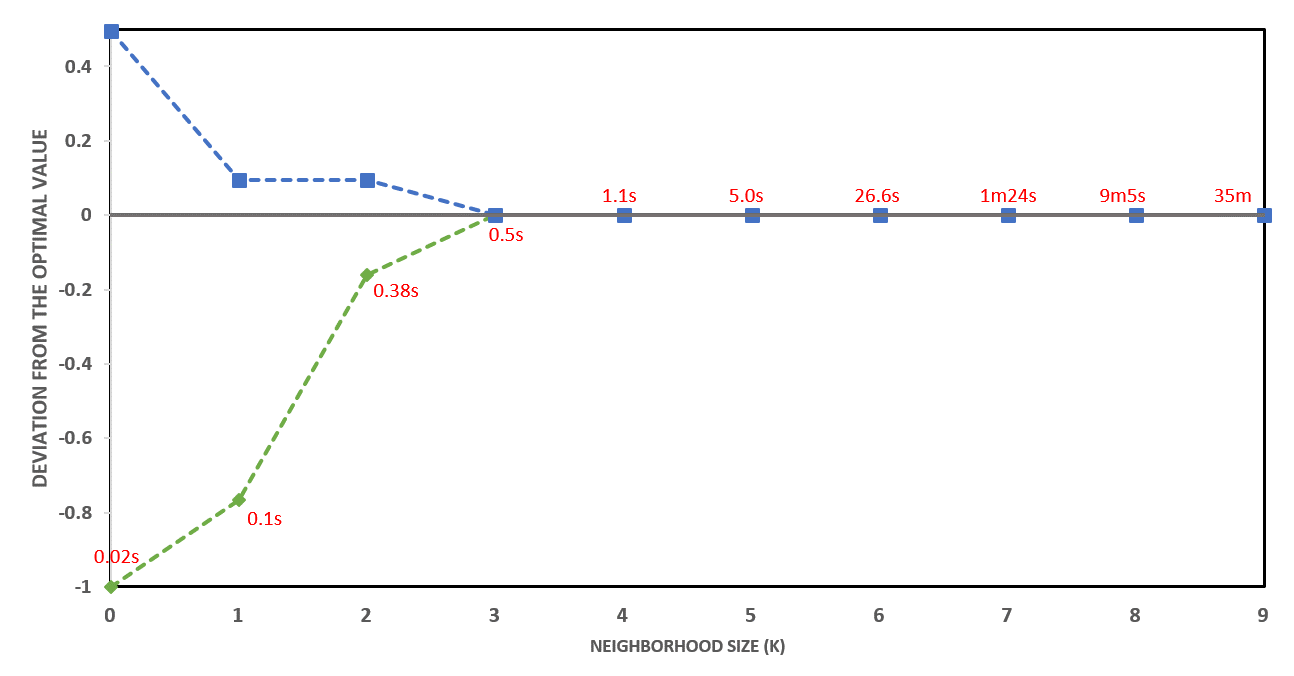
\includegraphics[width=\textwidth]{result_DNEG_n15k4j0.PNG}
		\caption{The results for $n=15$ with different $k$}
		\label{fig:n15k4j0}
	\end{figure}
\end{frame}

\begin{frame}{Computational results}  \tiny
	\begin{table}[htbp]
		\centering
		\begin{adjustbox}{width=\columnwidth, height=0.25\textheight, center}
			\begin{tabular}{rrrrccccrrrrrrrrrrrrrrrrrrr}
				\toprule
				&       & \multicolumn{1}{c}{CCLW} &       & \multicolumn{4}{c}{Mibs}      &       & \multicolumn{3}{c}{Single-level relaxation} &       & \multicolumn{4}{c}{$k=1$}       &       & \multicolumn{3}{c}{$k=2$} &       &       & \multicolumn{4}{c}{$k=3$} \\
				\cmidrule{3-3}\cmidrule{5-8}\cmidrule{10-12}\cmidrule{14-17}\cmidrule{19-22}\cmidrule{24-27}    \multicolumn{1}{c}{$n$} & \multicolumn{1}{c}{$r$} & \multicolumn{1}{c}{Time} &       & Unsolved & ObjL  & ObjU  & Time  &       & \multicolumn{1}{c}{ObjL} & \multicolumn{1}{c}{ObjU} & \multicolumn{1}{c}{Time} &       & \multicolumn{1}{c}{ObjL} & \multicolumn{1}{c}{ObjU} & \multicolumn{1}{c}{Time} & \multicolumn{1}{c}{Ext Time} &       & \multicolumn{1}{c}{ObjL} & \multicolumn{1}{c}{ObjU} & \multicolumn{1}{c}{Time} & \multicolumn{1}{c}{Ext Time} &       & \multicolumn{1}{c}{ObjL} & \multicolumn{1}{c}{ObjU} & \multicolumn{1}{c}{Time} & \multicolumn{1}{c}{Ext Time} \\
				\hline
				10    & 0     & 0.13  &       &       &       &       & 0.01  &       & 0     & 1.8   & 0.02  &       & 0.34  & 1.8   & 0.04  & 0.14  &       & 0.99  & 1.01  & 0.02  & 0.03  &       & 1     & 1     & 0.03  & 0.03 \\
				10    & 1     & 0.17  &       &       &       &       & 0.02  &       & 0     & 1.8   & 0.01  &       & 0.23  & 1.41  & 0.04  & 0.07  &       & 0.78  & 1.17  & 0.07  & 0.05  &       & 0.99  & 1     & 0.06  & 0.09 \\
				10    & 2     & 0.26  &       &       &       &       & 0.03  &       & 0     & 1.93  & 0.01  &       & 0.41  & 1.47  & 0.04  & 0.08  &       & 0.94  & 1.11  & 0.14  & 0.12  &       & 1     & 1     & 0.19  & 0.23 \\
				10    & 3     & 0.37  &       &       &       &       & 0.05  &       & 0     & 2.73  & 0.01  &       & 0.34  & 1.36  & 0.05  & 0.06  &       & 0.94  & 1.05  & 0.13  & 0.1   &       & 1     & 1.01  & 0.19  & 0.17 \\
				10    & 4     & 0.33  &       &       &       &       & 0.03  &       & 0     & 12.09 & 0.02  &       & 0.52  & 1.51  & 0.08  & 0.1   &       & 0.98  & 1.12  & 0.11  & 0.08  &       & 1.03  & 1.03  & 0.14  & 0.15 \\
				\hline
				30    & 0     & 1     &       &       &       &       & 2.98  &       & 0     & 1.54  & 0.01  &       & 0.06  & 1.38  & 0.1   & 0.07  &       & 0.7   & 1.12  & 0.18  & 0.2   &       & 1     & 1.01  & 0.42  & 0.35 \\
				30    & 1     & 8.17  &       & 6     & 0.95  & 1     & 212.99  &       & 0     & 1.82  & 0.01  &       & 0.1   & 1.45  & 0.11  & 0.08  &       & 0.73  & 1.13  & 0.22  & 0.15  &       & 0.97  & 1.01  & 1.01  & 0.92 \\
				30    & 2     & 19.99 &       & 8     & 0.81  & 1     & 249.20  &       & 0     & 1.94  & 0.01  &       & 0.19  & 1.46  & 0.17  & 0.09  &       & 0.73  & 1.09  & 0.19  & 0.16  &       & 0.97  & 1.02  & 1.29  & 0.89 \\
				30    & 3     & 15.46 &       & 10    & 0.81  & 1.03  &       &       & 0     & 2.54  & 0.01  &       & 0.31  & 1.62  & 0.16  & 0.12  &       & 0.8   & 1.16  & 0.27  & 0.21  &       & 0.99  & 1.01  & 1.16  & 0.64 \\
				30    & 4     & 0.33  &       & 5     & 0.82  & 1     & 203.42  &       & 0     & 3.82  & 0.01  &       & 0.67  & 1.52  & 0.18  & 0.16  &       & 1     & 1.03  & 0.28  & 0.21  &       & 1.01  & 1.01  & 0.62  & 0.38 \\
				\hline
				50    & 0     & 6.51  &       & 6     & 0.86  & 1     & 166.22  &       & 0     & 1.66  & 0.01  &       & 0.06  & 1.45  & 0.08  & 0.09  &       & 0.6   & 1.29  & 0.39  & 0.29  &       & 1.04  & 1.07  & 10.41 & 8.78 \\
				50    & 1     & 632.64 &       & 10    & 0.69  & 1     &       &       & 0     & 1.79  & 0.01  &       & 0.09  & 1.42  & 0.15  & 0.1   &       & 0.69  & 1.09  & 0.64  & 0.46  &       & 0.98  & 1.01  & 21.81 & 10.44 \\
				50    & 2     & 1422.86 &       & 10    & 0.49  & 1     &       &       & 0     & 2.05  & 0.01  &       & 0.18  & 1.42  & 0.23  & 0.09  &       & 0.64  & 1.07  & 0.64  & 0.45  &       & 0.98  & 1.01  & 22.14 & 11.69 \\
				50    & 3     & 1312.54 &       & 10    & 0.41  & 1.03  &       &       & 0     & 2.61  & 0.01  &       & 0.37  & 1.49  & 0.25  & 0.16  &       & 0.79  & 1.16  & 0.84  & 0.52  &       & 0.99  & 1.01  & 13.3  & 8.39 \\
				50    & 4     & 10.28 &       & 10    & 0.46  & 1.01  &       &       & 0     & 3.35  & 0.02  &       & 0.65  & 1.52  & 0.31  & 0.21  &       & 0.93  & 1.06  & 0.9   & 0.48  &       & 1     & 1     & 7.75  & 3.97 \\
				\hline
			\end{tabular}%
		\end{adjustbox}
	\end{table}%
	\begin{itemize}
		\item Average performance with 10 instances for each class
		\item The solution time of BP$_k$ is reported in seconds in column ``Time''
		\item The solution time of EBP$_k$ is reported in seconds in column ``Ext Time''
		\item In column ``ObjL'', the value is computed as the ratio between  best lower bound and optimal objective value
		\item In column ``ObjU'', the value is computed as the ratio between  best upper bound and optimal objective value
	\end{itemize}
\end{frame}



\section{Conclusion}
\begin{frame}{Conclusion}
Contributions:
\begin{itemize}
	\item Two single-level formulations for BP$_k$
	\item The single-level formulation for minimum spanning tree interdiction problem
	\item The computational study shows the efficiency of the proposed formulation
\end{itemize}
	\vspace{0.4cm}

	Future research:
	\begin{itemize}
		\item Advanced valid inequalities to solve BP$_k$
		\item Computational studies for general bilevel programs
	\end{itemize}
\end{frame}











\end{document}
